

%preamble

\documentclass[english]{article}
\usepackage{fullpage}
\usepackage[T1]{fontenc}
\usepackage[latin9]{inputenc}
\setlength{\parskip}{\medskipamount}
\setlength{\parindent}{0pt}

\usepackage{amsmath}
\usepackage{amssymb}
\usepackage{amsthm}
\usepackage{amsfonts}
\usepackage{graphicx}
\usepackage[all,arc,curve,frame]{xy}

\newcommand{\Nat}{\mathbb{N}}
\newcommand{\defeq}{:=}
\newcommand{\vect}[1]{\boldsymbol{#1}}

\renewcommand{\labelenumii}{\arabic{enumi}.\arabic{enumii}.}
\renewcommand{\labelenumiii}{\arabic{enumi}.\arabic{enumii}.\arabic{enumiii}.}
\renewcommand{\labelenumiv}{\arabic{enumi}.\arabic{enumii}.\arabic{enumiii}.\arabic{enumiv}.}



\usepackage{tikz}
\usetikzlibrary{arrows}

\begin{document}
\title{
 CS5811 Project Proposal:\\
 Search for Self-Stabilizing Protocols
}

\author{~Brandon~Crowley,~Alex~Klinkhamer, and~Mandy~Wang}
\maketitle


\section{Proposed Work}

Our group intends to use search techniques from AI to synthesize self-stabilization for protocols defined between finite-state machines.
A self-stabilizing protocol is guaranteed to eventually reach some global legitimate state from any illegitimate state, which could be caused by environmental factors or bad initialization.

In the spirit of keeping useful information near the top, a more detailed description of the problem is left until the end.

\subsection{AI Techniques}

The problem of finding a stabilizing protocol asks: {\em What, if any, set of process actions ensures the system will always converge to a legitimate state?}

We plan to use a backtracking algorithm with a good analogue of the Most-Constrained Variable heuristic paired with AC-3 to see how well the search performs.
This is not a classical constraint satisfaction problem, but we think the methods still apply.

Along the development process, we may find some other search methods to try.
It may be beneficial to also take process symmetry into account to narrow the search.

\subsection{State of the Art}

The addition of convergence to a non-stabilizing protocol has not yet enjoyed much practical application.
Currently, the most successful way of creating self-stabilizing protocols involves a lot of manual work.
We have not found any stabilizing protocol which was synthesized by a machine {\em before} being reasoned about by a human.

As far as we are aware, most automated approaches to adding convergence to non-stabilizing protocols use incomplete heuristics to achieve polynomial time bounds \cite{sycraft2008,ftsyn,taasFarahat12}.
Some of these apply to fault tolerance, of which stabilization is a special case.

One interesting approach formulates the invariant of a fault-intolerant program as a conjunction of constraints and satisfies them in order \cite{sssAbujaradK09}.
This approach has great results, but seems to involve a manual step in choosing good constraints.

Another nice approach for automating addition of fault tolerance deals with a purely symbolic algorithm \cite{icdcs07Borzoo}.
This result seems to exploit properties of fault tolerance which we cannot leverage for stabilization.
Even so, the paper deals with very large state spaces with fairly low memory utilization.

Binary decision diagrams (BDDs) are used heavily to combat the state explosion problem.
Instead of building an explicit global transition graph to check for cycles and reachability, BDD packages such as CUDD \cite{somenzi1998cudd} are used to represent the transitions symbolically.
A linear-time algorithm exists for cycle checking with BDDs \cite{sodaGentilini03}, like Tarjan's algorithm on an explcit graph.

\subsection{Contributions}

If one of these tools which relies on polynomial-time heuristics fails to find a solution, we cannot be sure if a solution exists or not.
For someone designing a protocol who {\em does not know} if a stabilizing version exists, this can be troublesome.
Therefore, our contribution is further exploration of complete methods for adding convergence.

\section{Tasks}

The following is a dependency graph of the tasks we plan to accomplish.
Edges with no arrows signify potentially bidirectional dependencies.
We have not estimated the amount of time each task will take, but we expect some tasks to be trivial, leaving time for additional experimentation.

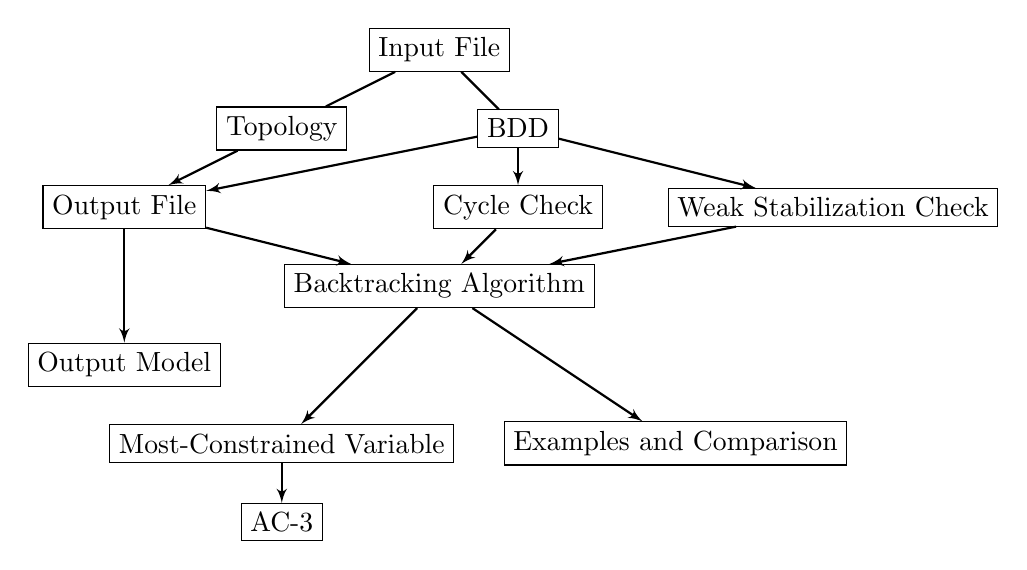
\begin{tikzpicture}[x=1cm,y=1cm]
 \tikzstyle{every node}=[draw]
 \tikzstyle{l} = [draw,-latex',thick]
 \tikzstyle{b} = [draw,thick]
 \draw
 node (Input) {Input File}
 (Input) ++(-2,-1) node (Topology) {Topology}
 (Input) ++(1,-1) node (BDD) {BDD}
 (Topology) ++(-2,-1) node (Output) {Output File}
 (Output) ++(0,-2) node (Model) {Output Model}
 (BDD) ++(4,-1) node (WS) {Weak Stabilization Check}
 (BDD) ++(0,-1) node (Cycle) {Cycle Check}
 (Input) ++(0,-3) node (Backtrack) {Backtracking Algorithm}
 (Backtrack) ++(-2,-2) node (MCV) {Most-Constrained Variable}
 (MCV) ++(0,-1) node (AC3) {AC-3}
 (Backtrack) ++(3,-2) node (Example) {Examples and Comparison}
 ;
 \path [b] (BDD) -- (Input);
 \path [b] (Input) -- (Topology);
 \path [l] (BDD) -- (WS);
 \path [l] (BDD) -- (Cycle);
 \path [l] (BDD) -- (Output);
 \path [l] (Topology) -- (Output);
 \path [l] (Output) -- (Model);
 \path [l] (Output) -- (Backtrack);
 \path [l] (Cycle) -- (Backtrack);
 \path [l] (WS) -- (Backtrack);
 \path [l] (Backtrack) -- (MCV);
 \path [l] (MCV) -- (AC3);
 \path [l] (Backtrack) -- (Example);
\end{tikzpicture}

\begin{description}
 \item[Input File]
  Read in a non-stabilizing protocol with a description of the system topology (read/write restrictions for each process) and set of legitimate states.
  The STSyn and SYCRAFT tools use the same input format, we can consult their parsing routines.
 \item[Topology]
  Create data structures to store the system description.
 \item[Output File]
  Output the synthesized protocol in some format.
 \item[BDD]
  Set up and learn how to store process actions in a BDD.
 \item[Weak Stabilization Check]
  Make a check to see if all illegitimate states have a path to the set of legitimate states.
 \item[Cycle Check]
  Make a check for cycles (livelocks) in the set of illegitimate states.
 \item[Backtracking Algorithm]
  Make a simple backtracking algorithm with no heuristics.
 \item[Output Model]
  Output a model of the synthesized protocol which can be verified as self-stabilizing by the Spin model checker.
  The exact format is already known, so this task is rather small.
 \item[Most-Constrained Variable]
  Use an analogue of the MCV heuristic in the backtracking algorithm.
 \item[AC-3]
  Perform an analogue of AC-3 after committing to include an action.
 \item[Examples and Comparison]
  We would like to try test using some well-known problems to see where the complexity limit lies for our algorithm.
\end{description}

\section{Software and Prior Work}

\subsection{STSyn}

STSyn \cite{taasFarahat12} is a utility which uses heuristics to synthesize a stabilizing protocol from a non-stabilizing version.
We can use its input file format and reference its code for proper cycle detection and backwards reachability algorithms using BDDs.

\subsection{SYCRAFT}

SYCRAFT \cite{sycraft2008} is a tool which synthesizes fault-tolerant protocols using some heuristics.
It may be useful to compare against, since the stabilization problem can be formulated as a fault tolerance problem.
Even so, it may perform poorly because stabilization is an edge-case of fault tolerance.

\subsection{BDD Package}

During the search process, we need to check for cycles and backwards reachability in the global transition graph.
The nodes of this graph represent states in the system and arcs represent transitions.
Due to the exponential nature of the state space, it quickly becomes infeasible to build an explicit transition graph.

Luckily, binary decision diagram (BDDs) offer symbolic methods for these checks.
The CUDD package paired with GLU seems to be the package of choice in the verification community, but we may favor a more accessible package like BuDDy or JINC.

\subsection{Model Checker}

To verify the generated protocol is correct, we can use the Spin model checker \cite{spin97}.
Simply, Spin verifies that any sequence of nondeterministic choices does not violate some set of assertions.
These nondeterministic choices can represent conditional statements and process execution interleaving.

So our approach will be to initialize all process variables to any value nondeterministically, then assert that a legitimate state is eventually reached.

\subsection{SAT Solver}

An unpublished tool exists which reduces the problem to SAT (in DIMACS format), which may be useful to compare against.
MiniSat could be used here, but plenty of others exist.

\section{Problem}

This final section describes self-stabilization and the problem of adding stabilization in greater detail.

\subsection{Example}
Before jumping into any technical description, let us consider the original token ring protocol Dijkstra used when introducing the concept of self-stabilization.
A token ring is used to give one process out of many an exclusive right, also known as distributed mutual exclusion.
Below is a ring of $6$ finite-state machines (processes).

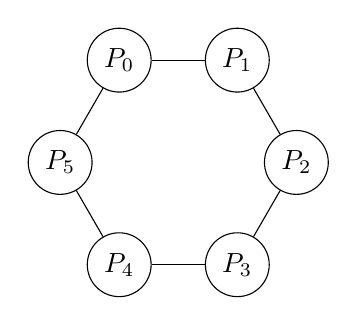
\begin{tikzpicture}[x=1.5cm,y=1.5cm]
 \tikzstyle{every node}=[draw,circle]
 \draw
 (0,0)      node (0) {$P_0$}
 ++(   0:1) node (1) {$P_1$}
 ++( -60:1) node (2) {$P_2$}
 ++(-120:1) node (3) {$P_3$}
 ++(-180:1) node (4) {$P_4$}
 ++(-240:1) node (5) {$P_5$}
 ;
 \draw (0) -- (1);
 \draw (1) -- (2);
 \draw (2) -- (3);
 \draw (3) -- (4);
 \draw (4) -- (5);
 \draw (5) -- (0);
\end{tikzpicture}

Each process $P_i$ holds a variable $x_i$ which ranges from $0$ to $6$ ($x_i\in\Nat_7$).
Each $P_i$ can read and write $x_i$ and can read $x_{i-1}$ (where subtraction is modulo $6$).
Note that each process can only read one of its neighbors, so we call this ring {\em unidirectional}.
At this point, we can see each $P_i$ has $49$ local states since $x_{i-1}$ and $x_i$ can each have $7$ different values.
That is, $\abs{\mathsc{Dom}(x_{i-1}) \times \mathsc{Dom}(x_i)} = \abs{\Nat_7\times \Nat_7} = 7 \cdot 7 = 49$.

The token ring provides mutual exclusion, granting an exclusive right when a process has a token.
$P_0$ is said to have a token when it sees $x_5 = x_0$.
Any other $P_i$ has a token when $x_{i-1} \neq x_i$.
Clearly for mutual exclusion to work, exactly one token must exist in the system, so we call these states with one token {\em legitimate} states.
The system is self-stabilizing if, for any illegitimate state (where either $0$ or more than $1$ tokens exist), the system will eventually reach a legitimate state.

Since these processes are finite-state machines, they have a condition which enables a local transition, or action, between states.
We allow a process to perform a read/write atomically.

Processes act as finite-state machines, where some condition enables an atomic transition between local states.
We use guarded commands to represent these local transitions.
A guarded command defines an {\em action} which a process can take when its {\em guard} evaluates to true.
The following guarded commands define a stabilizing protocol for Dijkstra's token ring of $6$ processes.
\[
\begin{array}{rrcl}
 P_0: & x_{5} = x_0 & \to & x_0 \defeq x_0 + 1 \modop{7}
\\ P_{i>0}: & x_{i-1} \neq x_i & \to & x_i \defeq x_{i-1}
\end{array}
\]

\subsection{Definitions}

\subsubsection{Invariant}

The set of legitimate states is defined by a state predicate, or boolean function over protocol variables, called an {\em invariant} which is commonly denoted by $I$.

In the case of the token ring, the invariant evaluates to true iff exactly one token exists in the ring.
\begin{eqnarray*}
 I & \equiv & (\exists i: \mathsc{Token?}(i)) \wedge (\forall i, j: i = j \vee \neg \mathsc{Token?}(i) \vee \neg \mathsc{Token?}(j))
\\ \mathsc{Token?}(i) & \equiv & (i = 0 \wedge x_5 = x_0) \vee (i \neq 0 \wedge x_{i-1} \neq x_i)
\end{eqnarray*}

\subsubsection{Closure}

We say that $I$ is closed under a protocol $p$ iff all transitions $(s_0, s_1)$ of $p$ with $s_0 \in I$ have $s_1 \in I$.
That is, closure holds iff $p$ never transitions from a legitimate state to an illegitimate state.
A stabilizing protocol preserves closure.

The token ring preserves closure since, if only one process has a token, it simply passes the token when it acts.
That is, if $P_0$ has the token, we know $x_0=x_1=\cdots=x_5$.
$P_0$ eventually increments $x_0$ which makes $x_5\neq x_0$ and $x_0\neq x_1$ which means $P_0$ becomes disabled without a token but $P_1$ has acquired the token!
Circulation of a single token continues indefinitely.

\subsubsection{Deadlock Freedom}

A deadlock is a state where no process is enabled.
In other words, in the global transition graph $p$ where nodes are states and arcs are transitions (caused by process actions), a deadlock is a node with no outgoing arc.
If a protocol has an illegitimate deadlock state, it will never converge to a legitimate state.
Thus, we see a stabilizing protocol must be deadlock free outside of the invariant.

In the token ring example, at least one process is always enabled.
Consider trying to disable all processes.
To disable $P_1,\dots,P_5$, we need $x_0=x_1=x_2=x_3=x_4=x_5$.
In this case, $P_0$ is enabled, therefore no deadlock can exist!

\subsubsection{Livelock Freedom}

A livelock is an execution which visits the same global state after some positive number of steps.
In other words, in the global transition graph $p$ where nodes are states and arcs are transitions (caused by process actions), a livelock is a directed cycle.
If a livelock exists amongst illegitimate states in a protocol being run under an unfair scheduling policy (or perhaps no scheduler), then a system may remain in the livelock indefinitely.
Of course if this is the case, a legitimate state will never be reached.

\subsubsection{Convergence}

Two definitions exist for convergence.
A protocol $p$ strongly converges to $I$ iff from every illegitimate state, all executions of $p$ bring the system to a state in $I$ after a finite number of steps.
A protocol $p$ weakly converges to $I$ iff from every illegitimate state, there exists an execution of $p$ which brings the system to a state in $I$ after a finite number of steps.

Simply put, a weak convergence allows livelocks whereas strong convergence does not.
It is customary to say ``convergence'' to mean ``strong convergence''.

\subsubsection{Stabilization}

A protocol $p_{ss}$ is strongly-stabilizing iff it has strong convergence to its invariant $I$ and is closed in $I$.
Similarly, a protocol $p_{ws}$ is weakly-stabilizing iff it has weak convergence to its invariant $I$ and is closed in $I$.

It is customary to say ``self-stabilizing'' or just ``stabilizing'' to mean ``strongly-stabilizing''.

\subsection{Synthesis}

If we wish to synthesize a stabilizing protocol $p_{ss}$ from a non-stabilizing version $p$, we must find a set of process actions which can be added to $p$ which ensure convergence to invariant $I$ and preserve closure in $I$.

A simple backtracking algorithm recursively adds process actions to resolve deadlocks outside of $I$.
If a livelock is created before all deadlocks are resolved, the search must backtrack since adding more actions will not resolve the livelock.
In other words, adding more arcs to the global transition graph will not resolve the directed cycle representing the livelock.



\bibliographystyle{plain}
\bibliography{bibliography}
\end{document}

